\documentclass[a4paper,12pt,openany]{book}
\usepackage{amsmath}
\usepackage{amssymb}

\usepackage{polski}
\usepackage[utf8]{inputenc}

\usepackage[pdftex,usenames,dvipsnames]{color}

\usepackage[pdftex,	pagebackref=false,draft=false,pdfpagelabels=false,pdfstartview=FitV,pdfstartpage=1,bookmarks=true,pdfauthor={Autor},pdftitle={Praca inżynierska},pdfsubject={Tytuł pracy},pdfkeywords={slowa kluczowe},unicode=true]{hyperref}   

\usepackage{extsizes}
\usepackage[a4paper,left=3.5cm,right=2.5cm,top=2.5cm,bottom=2.5cm]{geometry}
\usepackage{tocloft}
\usepackage{array}
\usepackage[format=hang,labelsep=period,labelfont={bf,small},textfont=small]{caption}
\usepackage{floatflt}
\usepackage{subfig}
\usepackage{graphicx}
\usepackage{here}
\usepackage{url}
\usepackage{enumerate}
\usepackage{multirow}
\usepackage{listings}
\usepackage{slantsc}

% ------------------------------------------------------------------------
% inne
% ------------------------------------------------------------------------
\usepackage{glossaries}

\usepackage{dashrule}
\usepackage{fancyhdr}
\usepackage{calc}
\usepackage{packages/zmienne}
\usepackage{packages/strona_tytulowa}
\usepackage{packages/oswiadczenie}
\usepackage{packages/karta_pracy}
\usepackage{packages/pusta_strona}
\usepackage{longtable}

\usepackage{indentfirst}

% ------------------------------------------------------------------------
% kodowanie czcionek
% ------------------------------------------------------------------------
\usepackage[T1]{fontenc}
\usepackage{lmodern}\normalfont %to load T1lmr.fd 

% ------------------------------------------------------------------------
% do algorytmów
% ------------------------------------------------------------------------

\usepackage{algorithm}
\usepackage{algorithmic}
\floatname{algorithm}{Algorytm}

% ------------------------------------------------------------------------
% do nonmeklatury
% ------------------------------------------------------------------------

\usepackage[section]{placeins}
\usepackage{nomencl}
\makenomenclature
\usepackage{makeidx}
\makeindex
\renewcommand{\nomname}{Spis ważniejszych symboli}
\makeatletter
    \def\numberline#1{\hb@xt@\@tempdima{#1.\hfil}}
    \renewcommand*\@seccntformat[1]{\csname the#1\endcsname.\enspace}
\makeatother

\makeatother
\def\nonumsection#1{
    \section*{#1}
    \addcontentsline{toc}{section}{#1}
    }
\def\nonumsubsection#1{
    \subsection*{#1}
    \addcontentsline{toc}{subsection}{#1}
    }
\reversemarginpar
\def\notka#1{
    \marginpar{\footnotesize{#1}}
    }

\newcommand{\myemptypage}{ \newpage  \thispagestyle{empty}~\newpage}

\lstdefinestyle{praca}{basicstyle=\scriptsize\ttfamily, 
								keywordstyle=\color{black}\bfseries,
								numbers=left, 
								stepnumber=1, 
								numberstyle=\tiny, 
								numbersep=10pt,
								extendedchars=true, 
								frame=tb}
\lstset{style=praca}

\setlength{\headheight}{15pt}
\pagestyle{fancy}
\renewcommand{\chaptermark}[1]{\markboth{#1}{}}
\renewcommand{\sectionmark}[1]{\markright{#1}{}}

\fancyhf{}
\fancyhead[LE,RO]{\thepage}
\fancyhead[RE]{\textit{\nouppercase{\leftmark}}}
\fancyhead[LO]{\textit{\nouppercase{\rightmark}}}

\fancypagestyle{plain}{ %
\fancyhf{}
\renewcommand{\headrulewidth}{0pt}
\renewcommand{\footrulewidth}{0pt}}

\frenchspacing
\setlength{\parskip}{1pt}
\linespread{1.5}
\setcounter{tocdepth}{3}
\setcounter{secnumdepth}{3}

\renewcommand{\figurename}{Rys.}
\renewcommand{\tablename}{Tab.}
\renewcommand{\lstlistingname}{Listing}
\renewcommand{\lstlistlistingname}{Spis listingów}

\bibliographystyle{unsrt}

\DeclareFontShape{T1}{lmr}{bx}{sc} { <-> ssub * cmr/bx/sc }{}
\DeclareFontShape{T1}{lmr}{bx}{scit}{<-> ssub * cmr/bx/scsl}{}


\author{Kacper Drapała}
\kierunek{Informatyka}
\grupa{41INF-SSI-NP}
\title{System do klasteryzacji dokumentów tekstowych}
\tytulAngielski{A system for clustering text documents}
\uczelnia{Uniwersytet Zielonogórski}
\wydzial{Wydział Informatyki, Elektrotechniki i Automatyki}
\praca{Praca dyplomowa}
\promotor{Dr inż. Marek Kowal}
\konsultant{}
\miasto{Zielona Góra}
\miesiac{Luty}
\rok{2018}
\dzien{13}
\mm{05}

\begin{document}
\pagenumbering{roman}

\thispagestyle{empty}
\stronatytulowa

\thispagestyle{empty}
\pustastrona
\newpage

\normalsize
\subsection*{Streszczenie}

Niniejsza praca przedstawia realizację projektu, którego celem jest opracowanie systemu, który w sposób nienadzorowany będzie w stanie skategoryzować dokumenty tekstowe na podstawie ich treści.

Na początku pracy przedstawiona została teoria dotycząca eksploracji danych. Opisana została ścieżka instalacji oraz konfiguracji środowiska pracy i wykorzystanego języka programowania. Omówiono możliwości wykorzystanych bibliotek do wstępnego przetwarzania i klasteryzacji dokumentów tekstowych oraz wykorzystanych w dalszej części metod i technik do ich obróbki. 

W kolejnej części znajdują się szczegółowe informacje dotyczące wybranych technologii do uzyskania zamierzonego celu. Wytłumaczone zostały poszczególne etapy przygotowania dokumentów tekstowych, m.in. czyszczenie, normalizacja oraz transformacja dokumentów tekstowych. 

Ostatni etap pracy poświęcono na badania eksperymentalne, których celem było zweryfikowanie skuteczności przygotowanego systemu. Badania przeprowadzono na zbiorze rzeczywistych dokumentów tekstowych pochodzących z ponad 2000 źródeł wiadomości.

\vspace{1cm}
\noindent\textbf{Słowa kluczowe:} sztuczna inteligencja, dokumenty tekstowe, klasteryzacja
\newpage
\tableofcontents
\newpage
 \listoffigures
\newpage
\listoftables
\newpage
\lstlistoflistings
\newpage

\newcounter{licznikStron}
\setcounter{licznikStron}{\value{page}}
\setcounter{licznikStron}{1}
\pagenumbering{arabic}
\setcounter{page}{\value{licznikStron}}

\chapter{Wstęp}
\section{Wprowadzenie}
Temat niniejszej pracy nie jest przypadkowy. Zastosowanie sztucznej inteligencji z dnia na dzień staje się coraz popularniejsze. Wielkie firmy wykorzystują ją do szybkiego rozpoznawania między innymi obrazów, dźwięków lub tekstów.

Inspiracją do napisania takiego systemu jest ciągła konieczność poprawiania algorytmów, szukających takich samych lub podobnych produktów ze sklepów internetowych w aktualnie wykonywanej pracy zawodowej. Problemem jest tu zbyt duża różnorodność dotycząca kategorii danych produktów. Towar z jednej kategorii ma w opisie inne informacje niż produkt z drugiej kategorii. System do klasteryzacji dokumentów tekstowych pozwoli na częściowe rozwiązanie tego problemu. Dzięki temu można w łatwy sposób wygenerować listę dokumentów tekstowych, które będą składać się z opisów, nazw, kategorii czy specyfikacji produktów. Następnie należałoby uruchomić algorytm, który pogrupuje dokumenty tekstowe w takie grupy, w których obiekty będą do siebie jak najbardziej podobne.

System ten będzie bardzo przydatny w branży E-Commerce, której pracownicy będą szybciej analizować ceny na rynku z różnych sklepów internetowych czy kategorii danych produktów. System sprawdzi się również do grupowania innych rodzajów dokumentów tekstowych. W poniższej pracy wykorzystam go do pogrupowania artykułów powiązanych ze sobą tematycznie, co przedstawię w kolejnych rozdziałach.


\section{Cel i zakres pracy}
Celem pracy jest utworzenie systemu, który na wejściu otrzymuję listę dokumentów tekstowych, a na wyjściu generuje grupy tych dokumentów dokonując selekcji poszczególnych dokumentów do grup na podstawie treści dokumentów. Oznacza to, że odległość pomiędzy dokumentem tekstowym z jednej grupy, a dokumentem z innej musi być jak największa, natomiast dla obiektów znajdujących się w tej samej grupie - jak najmniejsza.

Praca będzie swym zakresem obejmowała:
\begin{itemize}
    \item dokonanie przeglądu bibliotek do wstępnego przetwarzania i klasteryzacji dokumentów tekstowych,
    \item przygotowanie testowego zbioru dokumentów tekstowych,
    \item czyszczenie, normalizacja oraz transformacja dokumentów tekstowych,
    \item zastosowanie algorytmów klasteryzacji do budowy systemu klasteryzacji treści dokumentów tekstowych,
    \item wykonanie testów weryfikujących skuteczność opracowanego systemu.
\end{itemize}

\section{Struktura pracy}

Praca została podzielona na dwie części, teoretyczną oraz praktyczną. Część teoretyczna została zaprezentowana w rozdziale 2. W ramach tej części opisano metody przetwarzania dokumentów tekstowych, klasteryzacji oraz sposobów weryfikacji wyników. W rozdziale 3 zaprezentowano przykładowe wyniki dla metod, które opisano w rozdziale 2. Wyniki przedstawione są w formie rysunków oraz tabel wraz z komentarzem.
\chapter{Założenia projektowe}
\section{Eksploracja danych}
Eksploracja danych (ang. data mining) jest dziedziną nauki zajmującą się metodami pozyskiwania wiedzy z danych. Główne metody eksploracji danych to klasteryzacja i klasyfikacja danych, odkrywania wzorców asocjacji lub sekwencji, selekcja danych odstających. Algorytmy wykorzystywane do eksploracji danych pochodzą głównie z zakresu statystyki i uczenia maszynowego \cite{9783319141411}. Zwykle, aby wydobyć wiedzę np. z tekstu, musimy przetworzyć ogromne ilości danych. Źródłem tych danych mogą być strony WWW, artykuły w gazetach czy wiadomości E-mail. Dzięki eksploracji można wydobyć kolejno: informacje o konkretnym produkcie ze strony WWW, określić treść dokumentów tekstowych oraz określić czy dany E-mail jest spamem. 

\subsection{Klasteryzacja}
Klasteryzacja (grupowanie) inaczej nazywana jest klasyfikacją bez nadzoru. To metoda, dzięki której następuje pogrupowanie pewnego zbioru elementów w taki sposób, aby dane poszczególnych grup były do siebie jak najbardziej podobne. Grupowanie dąży do tego, aby odległości pomiędzy obiektami w jednej grupie były jak najmniejsze, natomiast odległość pomiędzy grupami obiektów - jak największa.

Na wykresie \figurename{\ref{fig:threeblobs}} osadzone są pewne obiekty. Trzema różnymi kolorami oznaczono przynależność do grupy. Możemy zaobserwować, że obiekty należące do tej samej grupy są skupione wokół siebie.

\begin{figure}[h!]
    \centering
    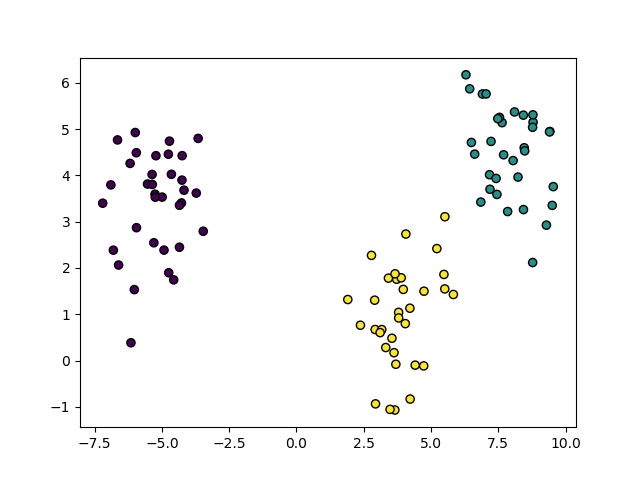
\includegraphics[scale=0.5]{Rysunki/Rozdzial2/4.png}
    \caption{Pogrupowane obiekty}
    \label{fig:threeblobs}
\end{figure}

\section{Python}
Python jest wieloplatformowym językiem programowania wysokiego poziomu. Został stworzony w celu zapewnienia dużej czytelności kodu źródłowego. Składnia tego języka jest przejrzysta dzięki zminimalizowaniu konstrukcji składniowych. Korzysta on z wcięć zamiast klamr, które oznaczają początek i koniec bloku instrukcji. Python rozwijany jest jako otwarty projekt (ang. open-source). Instalacja Pythona sprowadza się do pobrania instalatora oraz uruchomienia go, pamiętając, aby podczas instalacji zaznaczyć zgodę na dodanie przez instalator ścieżki Pythona do zmiennych środowiskowych systemu. Do realizacji niniejszej pracy wykorzystano Pythona w wersji 3.6.4.

%\begin{figure}[h!]
%  \centering
%  \subfloat{\label{fig:checkboxPython}
\includegraphics[width=0.40\textwidth]{Rysunki/Rozdzial2/1.png}}
%  \caption{Wymagane pole do zaznaczenia podczas instalacji oprogramowania}
%  \label{fig:srodowiskoPracyPy}
%\end{figure}

Weryfikacja poprawności instalacji języka programowania sprowadza się do uruchomienia programu z wiersza poleceń systemu Windows. Wówczas uruchamiamy program Python, w którym już teraz jest możliwość pisania mało skomplikowanych programów.

\begin{figure}[h!]
    \centering
    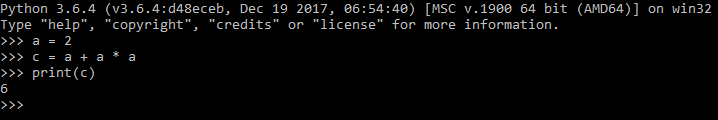
\includegraphics[scale=0.7]{Rysunki/Rozdzial2/5.png}
    \caption{Prosty przykład programu napisanego w języku Python w wierszu poleceń}
    \label{fig:simplePythonCmd}
\end{figure}

\section{Środowisko pracy}
Projekt powstał w środowisku Visual Studio Code w wersji 1.19.2 od firmy Microsoft oraz został napisany w języku Python w wersji 3.6.4. Środowisko to dostępne jest na platformach między innymi Windows, Linux i macOS. Środowisko jest darmowe oraz open-source.


Instalacja środowiska programistycznego na platformie Windows przebiega w bardzo prosty sposób. 
Pierwszym etapem jest instalacja Visual Studio Code, czyli edytora kodu, który wspiera najważniejsze operacje programowania. Tymi operacjami są na przykład debugowanie czy system kontroli wersji. Środowisko to zostało stworzone z myślą o szybkich cyklach pisania kodu oraz debugowania. Podczas instalacji należy zaznaczyć pole, które doda ścieżkę oprogramowania do zmiennych środowiskowych systemu operacyjnego.
\begin{figure}[h!]
  \centering
  \subfloat{\label{fig:checkboxVSC}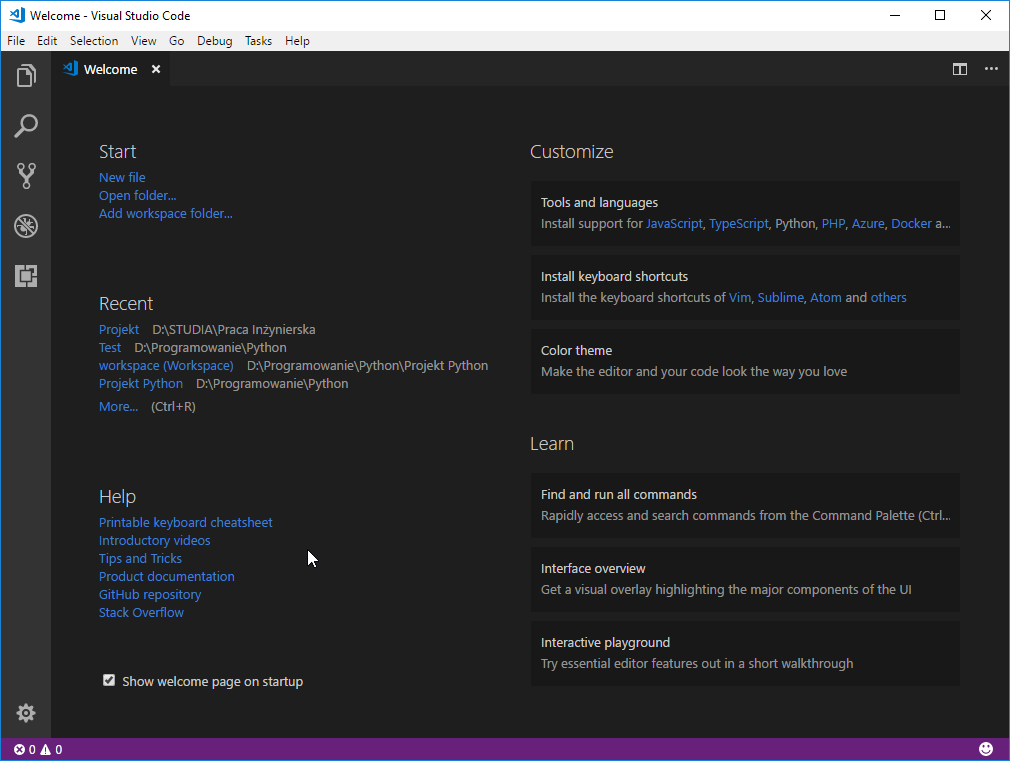
\includegraphics[width=0.9\textwidth]{Rysunki/Rozdzial2/srodowisko.png}}
  \caption{Interfejs środowiska Visual Studio Code}
  \label{fig:srodowiskoPracyVs}
\end{figure}

Kolejnym etapem jest konfiguracja wykorzystywanego środowiska, by móc uruchomić pisane w języku Python programy. W tym celu należy utworzyć nowy folder, który jest odpowiednikiem projektu w innych środowiskach programowania. Następnie stworzyć plik o rozszerzeniu \textit{.py}. W tym momencie pojawi się komunikat o zainstalowaniu rozszerzenia do Visual Studio Code, z dodatkami do języka Python, takimi jak:
\begin{itemize}
    \item formatowanie kodu,
    \item refaktoryzacja,
    \item pilnowanie składni języka,
    \item podpowiedzi.
\end{itemize}
Należy go zainstalować oraz zresetować Visual Studio Code klikając przycisk "Reload" obok dodanego rozszerzenia.


Następnie wchodzimy w zakładkę "Debug (Ctrl+Shift+D)" i klikamy na rozwijaną listę, po czym wybieramy opcję "Add Configuration...". W tym miejscu na górze programu wyświetlą się propozycje zainstalowanych w systemie środowisk. Po dodaniu konfiguracji Python, utworzy nowy folder o nazwie ".vscode" oraz plik "launch.json", w którym są wszystkie konfiguracje programu. Najważniejszą konfiguracją ze wszystkich jest ta położona na samej górze z nazwą "Python", ponieważ bez niej nie będziemy w stanie uruchamiać programów. Ostatnim elementem konfiguracji jest dodanie ścieżki dostępu do języka programowania. W zakładce "Explorer (Ctrl+Shift+E)" należy kliknąć prawym przyciskiem myszy i wybrać "Open Folder Settings". Utworzy się nowy plik w folderze ".vscode" o nazwie "settings.json", w którym są wszelkie opcje projektu. Po uruchomieniu tego pliku klikamy po prawej stronie "Workspace Settings", gdzie podajemy ścieżkę do programu Python.

\begin{figure}[h!]
    \centering
    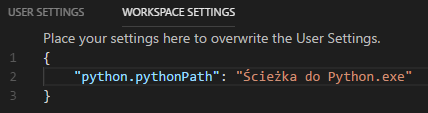
\includegraphics{Rysunki/Rozdzial2/3.png}
    \caption{Absolutna ścieżka do zainstalowanego programu Python.exe}
    \label{fig:pythonPath}
\end{figure}

Ostatnim krokiem jest weryfikacja, czy wszystko zostało poprawnie skonfigurowane. W tym celu wystarczy otworzyć stworzony wcześniej plik z rozszerzeniem \textit{.py} i napisać pierwsze standardowe polecenie "print('Hello World!')".

\newpage
\section{Biblioteki do wstępnego przetwarzania dokumentów tekstowych}
Aby zrealizować zaplanowane zadanie klasteryzacji dokumentów konieczne jest wstępne przetworzenie dokumentów tekstowych do postaci akceptowalnej przez procedury klasteryzacji. Język Python oferuje szereg bibliotek, które wspomagają realizację tych procesów. Najczęściej wykorzystywane do takich zadań biblioteki to Scikit-learn \cite{scikit-learn} oraz Natural Language Toolkit \cite{Loper02nltk:the}.

\subsection{Scikit-learn}
Scikit-learn jest darmową biblioteką do wykonywania czynności związanych z uczeniem maszynowym. Wprowadza wiele rozwiązań, jak: algorytmy klasyfikacji, regresji czy klasteryzacji. 

Biblioteka wymaga dodatkowo kilka innych modułów by działać poprawnie. Tymi modułami są:
\begin{itemize}
    \item NumPy w wersji wyższej bądź równej 1.8.2
    \item SciPy w wersji wyższej bądź równej 0.13.3
\end{itemize}

Instalacja bibliotek odbywa się z wiersza poleceń. Istnieją dwa sposoby realizacji tej procedury. Pierwszy z nich polega na uruchomieniu wiersza poleceń z samego Windowsa. W drugim instalacja odbywa się poprzez Terminal w Visual Studio Code, który ma wbudowaną w sobie integrację z Windows PowerShell. Jest to odpowiednik wiersza poleceń.

Kolejnym etapem jest instalacja wymaganych modułów dla języka Python. Instalację można przeprowadzić z wykorzystaniem menadżera pakietów "pip" wydając następujące polecenia: "pip install {nazwa modułu}", dla wyżej wymienionych bibliotek:
\lstinputlisting[label={lst:2},caption={Instalacja wymaganych modułów z podaniem wersji}, language=python, showstringspaces=false]{Algorytmy/Rozdzial2/pipInstall.py}

Aby zainstalować najnowsze wersje tych bibliotek
\lstinputlisting[label={lst:3},caption={Instalacja wymaganych modułów z najnowszej wersji}, language=python, showstringspaces=false]{Algorytmy/Rozdzial2/pipInstallNewest.py}

\subsection{Natural Language Toolkit}
NLTK jest narzędziem wspomagającym pisanie programów do przetwarzania języka naturalnego. Biblioteka dostarcza wiele istotnych dodatków, takich jak klasyfikacja, tokenizacja czy stemming (szczegółowy opis tych operacji zaprezentowane w podpunkcie \ref{prepareDocs}).

NLTK jest projektem otwartym (ang. open-source). Jego instalacja przebiega w taki sam sposób co instalacja Scikit-learn. Należy uruchomić wiersz poleceń lub Terminal i wykorzystać do tego programu "pip".
\lstinputlisting[label={lst:4},caption={Instalacja biblioteki NLTK z najnowszej wersji}, language=python, showstringspaces=false]{Algorytmy/Rozdzial2/pipInstallNLTK.py}

Przetestowanie instalacji tej biblioteki należy wykonać poprzez uruchomienie programu "python" z wiersza poleceń lub Terminala w środowisku Visual Studio Code, po czym uruchomić polecenia (\ref{lst:5})
\lstinputlisting[label={lst:5},caption={Weryfikacja poprawności instalacji biblioteki NLTK}, language=python, showstringspaces=false]{Algorytmy/Rozdzial2/importnltk.py}

Wywołanie metody "download()" z pakietu "nltk" spowoduje pojawienie się menadżera ze wszystkimi dodatkami tej biblioteki, "NLTK Downloader", dzięki któremu w łatwy sposób można zainstalować potrzebne dodatki.
\begin{figure}[h!]
    \centering
    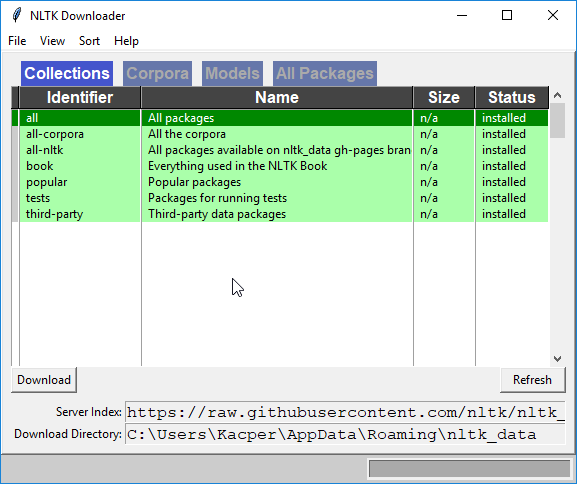
\includegraphics[scale=0.7]{Rysunki/Rozdzial2/6.png}
    \caption{NLTK Downloader}
    \label{fig:nltkdownloader}
\end{figure}

\section{Przygotowanie dokumentów tekstowych} \label{prepareDocs}
Zbyt duża różnorodność w dokumentach tekstowych może sprawić więcej problemów niż początkowo sądzimy. Długie oraz zbędne słowa czy znaki są powszechne niemal w każdych dokumentach tekstowych. Dlatego niezbędne jest wstępne przetworzenie tekstu na potrzeby klasteryzacji, tak by działała jak najkorzystniej. Przygotowywanie dokumentów można podzielić na kilka etapów, które przedstawiono w kolejnych podpunktach.

    \subsection{Tokenizacja} \label{sec:tokenizacja}
    Tokenizacja jest to transformacja dokumentu tekstowego w taki sposób, aby rozdzielić go na pojedyncze słowa. Zazwyczaj w tym momencie używana jest tokenizacja po białych znakach (ang. whitespace). Na zadanym dokumencie tekstowym jest wykonywana operacja dzielenia tekstu w miejscach spacji, nowych linii czy tabulatorów.
    
    Uruchomienie skryptu z listingu \ref{lst:6} podzieli nasz tekst w długą listę słów oraz wypisze 100 pierwszych.
    \lstinputlisting[label={lst:6},caption={Dzielenie tekstu po białych znakach}, language=python, showstringspaces=false, breaklines=true]{Algorytmy/Rozdzial2/splitByWS.py}
    
    Drugi sposób na podzielenie tekstu na części, to skorzystanie z wcześniej omówionej biblioteki Natural Language Toolkit. Biblioteka ta udostępnia gotową metodę do tokenizacji dokumentów tekstowych.
    
    \lstinputlisting[label={lst:7},caption={Dzielenie tekstu z wykorzystaniem biblioteki NLTK}, language=python, showstringspaces=false, breaklines=true]{Algorytmy/Rozdzial2/splitByNLTK.py}
    
    
    Różnice pomiędzy dwoma sposobami tokenizacji są niewielkie. 
    O ile pierwszy sposób rozróżnił słowa po znakach białych, to drugi rozdzielił je dodatkowo od znaków interpunkcyjnych.
    
    
    \subsection{Czyszczenie} \label{sec:czyszczenie}
    Czyszczenie dokumentów tekstowych polega na usunięciu niepotrzebnych elementów dokumentu tekstowego. Takimi elementami są: znaki interpunkcyjne, liczby i wyrazy znajdujące się na stop liście (ang. stopwords). 
    
    Python dostarcza nam gotową listę znaków interpunkcyjnych.
    \lstinputlisting[label={lst:8},caption={Lista wszystkich znaków interpunkcyjnych}, language=python, showstringspaces=false, breaklines=true]{Algorytmy/Rozdzial2/punctuation.py}
    
    Dzięki temu jesteśmy w stanie w łatwy sposób usunąć z tekstu wszystkie znaki interpunkcyjne. Python posiada również wbudowaną metodę "isalpha()", która zwraca wartość prawdziwą tylko wtedy, kiedy wszystkie znaki w tekście należą do zbioru znaków alfanumerycznych.
    
    \lstinputlisting[label={lst:9},caption={Czyszczenie dokumentu tekstowego wykorzystując tokeny z \ref{lst:7}}, language=python, showstringspaces=false, breaklines=true]{Algorytmy/Rozdzial2/cleaning.py}    
    Czyszczenie dokumentu tekstowego z elementów znajdujących się na stop liście (ang. stopwords), również można wykonać za pomocą biblioteki NLTK. Dostarcza ona predefiniowane stop listy w różnych językach. 
    \newpage
    \lstinputlisting[label={lst:10},caption={Kasowanie słów zawartych na stop liście}, language=python, showstringspaces=false, breaklines=true]{Algorytmy/Rozdzial2/stopwords.py}
    
    Istnieje również możliwość wygenerowania własnej stop listy na podstawie analizowanych dokumentów tekstowych. Zwykle taką listę generuje się zliczając ilość unikalnych słów we wszystkich dokumentach tekstowych, a następnie uznając te najbardziej popularne za słowa, które nie są istotne do klasyfikacji dokumentów. Ważnym elementem w tym procesie, jest wyznaczenie progu ilości wystąpień słowa, od którego zależy czy jest ono istotne czy nie.
    
    \subsection{Normalizacja} \label{sec:normalizacja}
    Normalizację (ang. normalization) konkretnych słów w dokumencie tekstowym można wykonać na wiele różnych sposobów. Zwykle polega ona na przyjęciu pewnego wzorca normalizacji dla całego dokumentu i zastosowaniu go do wszystkich słów w tekście. Jedną z metod normalizacji jest zwykła zamiana wszystkich słów w dokumencie na słowa z małymi literami (ang. lowercase) \cite{normalizeText}. Kolejnym krokiem jest normalizacja dat. Zapis dat w różnych częściach świata jest różny \cite{wiki:Date_format_by_country}. Jednak każdy miesiąc posiada swój unikalny skrót \cite{skrotyMiesiecy}, który należałoby znormalizować, czyli zamienić na pełne nazwy miesięcy. 
    
    Ostatnim etapem normalizacji jest stemming. Pierwsze próby zastosowania algorytmu stemmingu zostały zaproponowane w latach 60. XX wieku. Słowa o takim samym znaczeniu, które zapisane są na kilka różnych sposobów mogą być poddane stemmingowi. Proces ten kasuje końcówki fleksyjne ze słów w dokumencie tekstowym pozostawiając tylko część słowa zwaną rdzeniem. Można wyróżnić kilka rodzajów algorytmów stemmingu:
    \begin{itemize}
        \item Lancaster Stemmer,
        \item Snowball Stemmer,
        \item Porter Stemmer.
    \end{itemize}
    
    \lstinputlisting[label={lst:11},caption={Zastosowanie powyższych rodzajów stemmingu}, language=python, showstringspaces=false, breaklines=true]{Algorytmy/Rozdzial2/stemming.py}
    \newpage
    \subsection{TF-IDF} \label{sec:tfidf}
        Ważnym elementem grupowania dokumentów tekstowych, jest dobór odpowiednich cech opisujących dokument. Cechy ekstrachowane są z dokumentów tekstowych w ten sposób, aby dokumenty o podobnej treści uzyskiwały podobne wektory wartości cech. Dokumenty tekstowe o treściach różniących się od siebie powinny zostać opisane różnymi wektorami wartości cech.
        
        $TF-IDF$ (ang. TF - term frequency, IDF - inverse document frequency) jest klasyczną metodą, dzięki której możliwe jest przypisywanie wag poszczególnym słowom kluczowym opisującym dokument tekstowy.
        \begin{equation}
            \begin{bmatrix}
            $$w_{d_1t_1}$$ & . & . & $$w_{d_nt_1}$$\\ 
            . & . &  & .\\ 
            . &  & . & .\\ 
            $$w_{d_1t_n}$$ & . & . & $$w_{d_nt_n}$$
            \end{bmatrix}
        \end{equation}
        gdzie $w_{d_1t_1}$ to obliczona waga słowa $t_1$ w dokumencie $d_1$.
        
        
        Aby wyznaczyć wagi dla dokumentu tekstowego i policzyć współczynnik $TF-IDF$ należy w pierwszej kolejności obliczyć miary:
        \begin{itemize}
            \item częstotliwości występowania wyrażeń (ang. term frequency - $TF$) - $TF(t_i, d)$ - liczba wystąpień słowa $t_i$ w dokumencie d,
            \item częstotliwości dokumentów (ang. document frequency) - $DF(t_i)$ - liczba dokumentów tekstowych, w których istnieje słowo $t_i$,
            \item odwrotnej częstości dokumentu (ang. inverse document frequency - $IDF$) - $IDF(t_i) = 1+\ln{\left(\frac{|D|}{DF(t_i)}\right)}$ \cite{tfidf} gdzie |D| to liczba wszystkich dokumentów tekstowych,
        \end{itemize}
        $TF-IDF$ jest iloczynem miar $TF$ oraz $IDF$. 
        Przykładowo dla podanych poniżej trzech dokumentów tekstowych:
        \begin{itemize}
            \item $d1$ = The game of life is a game of everlasting learning,
            \item $d2$ = The unexamined life is not worth living,
            \item $d3$ = Never stop learning
        \end{itemize} należy na samym początku policzyć "term frequency", czyli ilość występowania danego słowa w dokumencie tekstowym. Drugą istotną rzeczą w tym etapie jest znormalizowanie $TF$. Normalizacja odbywa się za pomocą wzoru:
        \begin{equation}
            NTF(t_i, d) = \frac{TF(t_i, d)}{|C_d|}
        \end{equation}
        gdzie $|C_d|$ to ilość słów w dokumencie tekstowym.
        
        
        \begin{table}[h!]
            \centering
            \caption{Obliczone wartości $TF(t_i, d1)$ i $NTF(t_i, d1)$}
            \label{tfd1}
            \begin{tabular}{|l|l|l|l|l|l|l|l|l|}
            \hline
            $d1$ & the & game & of & life & is & a & everlasting & learning \\ \hline
            $TF(t_i, d1)$        & 1   & 2    & 2  & 1    & 1  & 1 & 1           & 1        \\ \hline
            $NTF(t_i, d1)$ & 0.1 & 0.2 & 0.2 & 0.1 & 0.1 & 0.1 & 0.1 & 0.1 \\ \hline
            \end{tabular}
        \end{table}
        
        \begin{table}[h!]
            \centering
            \caption{Obliczone wartości $TF(t_i, d2)$ i $NTF(t_i, d2)$}
            \label{tfd2}
            \begin{tabular}{|l|l|l|l|l|l|l|l|}
            \hline
            $d2$            & the & unexamined & life & is & not & worth & living \\ \hline
            $TF(t_i, d2)$ & 1   & 1          & 1    & 1  & 1   & 1     & 1      \\ \hline
            $NTF(t_i, d2)$ & 0.1428 & 0.1428 & 0.1428 & 0.1428 & 0.1428 & 0.1428 & 0.1428 \\ \hline
            \end{tabular}
        \end{table}

        \begin{table}[h!]
            \centering
            \caption{Obliczone wartości $TF(t_i, d3)$ i $NTF(t_i, d3)$}
            \label{tfd3}
            \begin{tabular}{|l|l|l|l|}
            \hline
            $d3$            & never & stop & learning \\ \hline
            $TF(t_i, d3)$ & 1     & 1    & 1        \\ \hline
            $NTF(t_i, d3)$ & 0.3333 & 0.3333 & 0.3333  \\ \hline
            \end{tabular}
        \end{table}
        \newpage
        Kolejnym krokiem jest policzenie współczynnika $IDF$ dla każdego termu ze wszystkich dokumentów tekstowych. Ilość wszystkich dokumentów jest równa 3, stąd
        \begin{equation}
            |D| = 3
        \end{equation}
        
        Korzystając ze wzoru
        \begin{equation}
            IDF(t_i) = 1+\ln{\left(\frac{|D|}{DF(t_i)}\right)}
        \end{equation}
        \begin{table}[h!]
            \centering
            \caption{Wartości współczynnika IDF dla wszystkich termów}
            \label{idf}
            \begin{tabular}{|l|l|}
            \hline
            Termy       & $IDF$     \\ \hline
            the         & 1.40546 \\ \hline
            game        & 2.09861 \\ \hline
            of          & 2.09861 \\ \hline
            life        & 1.40546 \\ \hline
            is          & 1.40546 \\ \hline
            a           & 2.09861 \\ \hline
            everlasting & 2.09861 \\ \hline
            learning    & 1.40546 \\ \hline
            unexamined  & 2.09861 \\ \hline
            not         & 2.09861 \\ \hline
            worth       & 2.09861 \\ \hline
            living      & 2.09861 \\ \hline
            never       & 2.09861 \\ \hline
            stop        & 2.09861 \\ \hline
            \end{tabular}
        \end{table}
        
        Ostatnim krokiem jest policzenie dla wszystkich termów współczynników $TF-IDF$. Można zauważyć, że czym większa obliczona waga, tym większa istotność danego słowa w dokumencie, dlatego też uważa się, że termy, które mają największą wagę w danym dokumencie tekstowym, są tymi cechami, które dosyć dobrze opisują jego tematykę. Zaletą współczynnika $TF-IDF$ jest to, że przy odróżnianiu jednego dokumentu tekstowego od innych, wpływ ma nie tylko częstość występowania w nim danego słowa, ale też występowanie tego słowa w innych dokumentach. 
        \begin{table}[h!]
            \centering
            \caption{Wartości współczynnika $TF-IDF$ dla dokumentów tekstowych}
            \label{tfidf}
            \begin{tabular}{|l|l|l|l|}
            \hline
            Termy       & $d1$       & $d2$       & $d3$       \\ \hline
            the         & 0.140546 & 0.200699 & 0        \\ \hline
            game        & 0.419722 & 0        & 0        \\ \hline
            of          & 0.419722 & 0        & 0        \\ \hline
            life        & 0.140546 & 0.200699 & 0        \\ \hline
            is          & 0.140546 & 0.200699 & 0        \\ \hline
            a           & 0.209861 & 0        & 0        \\ \hline
            everlasting & 0.209861 & 0        & 0        \\ \hline
            learning    & 0.140546 & 0        & 0.468439 \\ \hline
            unexamined  & 0        & 0.299681 & 0        \\ \hline
            not         & 0        & 0.299681 & 0        \\ \hline
            worth       & 0        & 0.299681 & 0        \\ \hline
            living      & 0        & 0.299681 & 0        \\ \hline
            never       & 0        & 0        & 0.699466 \\ \hline
            stop        & 0        & 0        & 0.699466 \\ \hline
            \end{tabular}
        \end{table}
        
        \newpage
        Policzenie $TF-IDF$ za pomocą Pythona sprowadza się do wykorzystania biblioteki Scikit-learn posiadającej w sobie klasę TfidfVectorizer, która na wejściu otrzymuje listę dokumentów, a następnie zwraca wszystkie wagi słów. Klasa ta posiada również dużo parametrów, jak "stopwords='english'", która wyklucza wszystkie słowa zawierające się na stop liście.
        
        \lstinputlisting[label={lst:12},caption={Przykład kodu wykorzystanego do policzenia $TF-IDF$ dla dokumentów tekstowych}, language=python, showstringspaces=false, breaklines=true]{Algorytmy/Rozdzial2/tfidf.py}
        \newpage
        
\section{Klasteryzacja danych}
    \subsection{Algorytm k-means} \label{sec:kmeans}
    Algorytm k-Means jest wykorzystywany do partycjonowania danych obserwacyjnych w predefiniowaną ilość klastrów. Algorytm opracowany przez J MacQueen-a (patrz \cite{macqueen1967}) rozpoczyna się od losowego rozmieszczenia zestawu środków klastrów ($\mu$) uważanych za środki klastrów. Podczas każdego kroku aktualizacji wszystkie obserwacje $x$ są przypisywane do najbliższego punktu środkowego (patrz równanie \ref{eqn:kmeansKrok}). W standardowym algorytmie każda obserwacja $x$ (punkt z danymi) jest przypisana do jednego klastra. Jeśli kilka środków klastrów ma taką samą odległość do obserwacji $x$, wtedy punkt jest przypisywany losowo do wybranego klastra z puli równoodległych klastrów.
    
    Przydzielenie jednej obserwacji do klastra, którego średnia ma najmniejszą kwadratową odległość euklidesową. 
    \begin{equation}
        S_i = \big \{ x_p : \big \| x_p - \mu_i \big \|^2 \le \big \| x_p - \mu_j \big \|^2 \ \forall j, 1 \le j \le k \big\}
        \label{eqn:kmeansKrok}
    \end{equation}
    gdzie: $S_i$ to zbiór punktów należących do $i-tego$ klastra, $x_p$ to wektor cech opisujący dokument tekstowy, $\mu_i$ to środek $i-tego$ klastra.
    
    Następnie środki klastrów są aktualizowane poprzez obliczenie średniej ze wszystkich obserwacji przypisanych do danego klastra (\ref{eqn:kmeans_update_step}):

    \begin{equation}
        \mu_i = \frac{1}{|S_i|} \sum_{x_j \in S_i} x_j
        \label{eqn:kmeans_update_step}
    \end{equation}
    gdzie: $\mu_i$ to środek $i-tego$ klastra, $|S_i|$  ilość elementów w $i-tym$ klastrze, $x_j$ wektor cech opisujący dokument należący do $S_i$.
    
    Proces aktualizacji środków klastrów powtarza się do momentu, aż wszystkie obserwacje przestają zmieniać przynależność do klastrów. Na zaprezentowanych poniżej rysunkach, przedstawiono przebieg przykładowego procesu klasteryzacji. W pierwszej iteracji położenie środków klastrów jest określane losowo, a następnie wszystkie punkty danych są przypisywane do najbliższych klastrów.
    
    W drugiej iteracji położenie środków klastrów jest aktualizowane na podstawie przypisanych do klastra obserwacji. Nowe środki obliczamy, jako średnia wszystkich obserwacji przydzielonych do danego klastra. 
    Ostatnią iteracją jest kolejna aktualizacja środków klastrów. Ponieważ w tej iteracji nie zmieniła się przynależność obserwacji do klastrów, to algorytm na tym etapie kończy swoje działanie.
    
    \begin{figure}[h!]
        \centering
        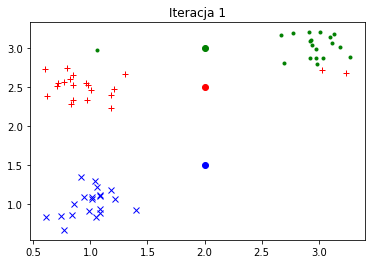
\includegraphics[width=0.6\linewidth]{Rysunki/Rozdzial2/iteracja1.png}
        \caption{Algorytm k-Means: Inicjalizacja algorytmu poprzez losowe rozmieszczenie środków klastrów i wyznaczenie przynależność punktów danych do klastrów}
        \label{fig:kmeans:iteration01}
    \end{figure}

    \begin{figure}[h!]
        \centering
        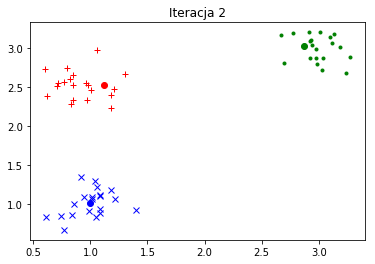
\includegraphics[width=0.6\linewidth]{Rysunki/Rozdzial2/iteracja2.png}
        \caption{Algorytm k-Means: druga iteracja - aktualizacja pozycji środków klastrów oraz ponowne przydzielenie obserwacji do klastrów}
        \label{fig:kmeans:iteration02}
    \end{figure}
    \newpage
    \begin{figure}[h!]
        \centering
        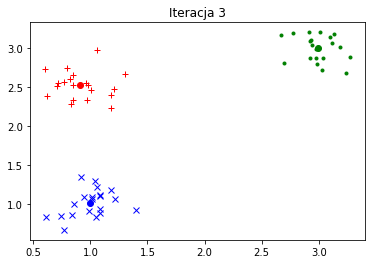
\includegraphics[width=0.6\linewidth]{Rysunki/Rozdzial2/iteracja3.png}
        \caption{k-Means: trzecia iteracja - aktualizacja pozycji środków klastrów}
        \label{fig:kmeans:iteration03}
    \end{figure}
    Głównym problemem algorytmu k-Means jest jego zależność od początkowo wybranych pozycji środków klastrów. Dwa centra mogą znaleźć tą samą grupę i podzielić się obserwacjami, w momencie kiedy dla dwóch środków klastrów przydzieli się punkty danych z tej samej grupy. Kolejne iteracje będą powielały błąd stworzony na samym początku działania algorytmu. Błędne początkowe położenie środków klastrów pokazano na rysunku \ref{fig:kmeans_bad1}.
    \newpage
    \begin{figure}[h!]
        \centering
    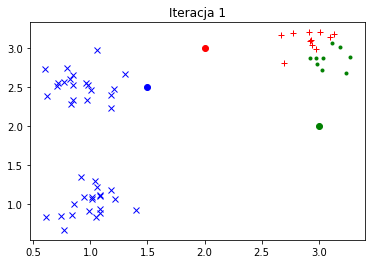
\includegraphics[width=0.6\linewidth]{Rysunki/Rozdzial2/zlaiteracja1.png}
    \caption{Algorytm k-Means: Złe początkowe pozycje środków klastrów}
    \label{fig:kmeans_bad1}
    \end{figure}
    
    \begin{figure}[h!]
        \centering
    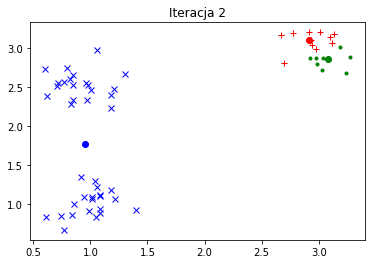
\includegraphics[width=0.6\linewidth]{Rysunki/Rozdzial2/zlaiteracja2.png}
    \caption{Algorytm k-Means: Aktualizacja środków klastrów oraz ponowne przydzielenie punktów danych}
    \label{fig:kmeans_bad2}
    \end{figure}

    k-Means najlepiej radzi sobie z klasteryzacją danych w których, klastry są mniej więcej równej wielkości i mają kolisty kształt.
    \newpage
    
    \subsection{DBSCAN}
    Algorytm DBSCAN (ang. Density Based Spatial Clustering of Application with Noise) jest jednym z algorytmów typu gęstościowego. Został zaprezentowany w 1996 roku przez czterech naukowców: Martin Ester, Hans-Peter Kriegel, Jörg Sander oraz Xiaowei Xu \cite{dbscan}. Działanie algorytmu wymaga podania dwóch parametrów: maksymalnego promienia sąsiedztwa $Eps$ i minimalnej ilości punktów oznaczanej jako $minPts$. Algorytm rozpoczyna działanie od wybrania dowolnego punktu w zbiorze danych. Jeśli w w maksymalnym promieniu sąsiedztwa znajduje się minimalna ilość punktów w odległości od punktu początkowego to znalezione punkty są przydzielane do jednego klastra. 
    
    Algorytm kontynuuje rozbudowywanie klastra do momentu, w którym nie istnieje $minPts$ w obrębie $Eps$ od najbardziej wysuniętego punktu w klastrze.
    
    W przeciwieństwie do algorytmu k-Means, algorytm DBSCAN potrafi dokonać klasteryzacji danych tworzących skupiska o różnych kształtach i wielkościach. Ponadto algorytm potrafi klasteryzować zbiory danych, które zawierają się w innej grupie co ilustruje rysunek \ref{fig:dbscan}
    \begin{figure}[h!]
        \centering
    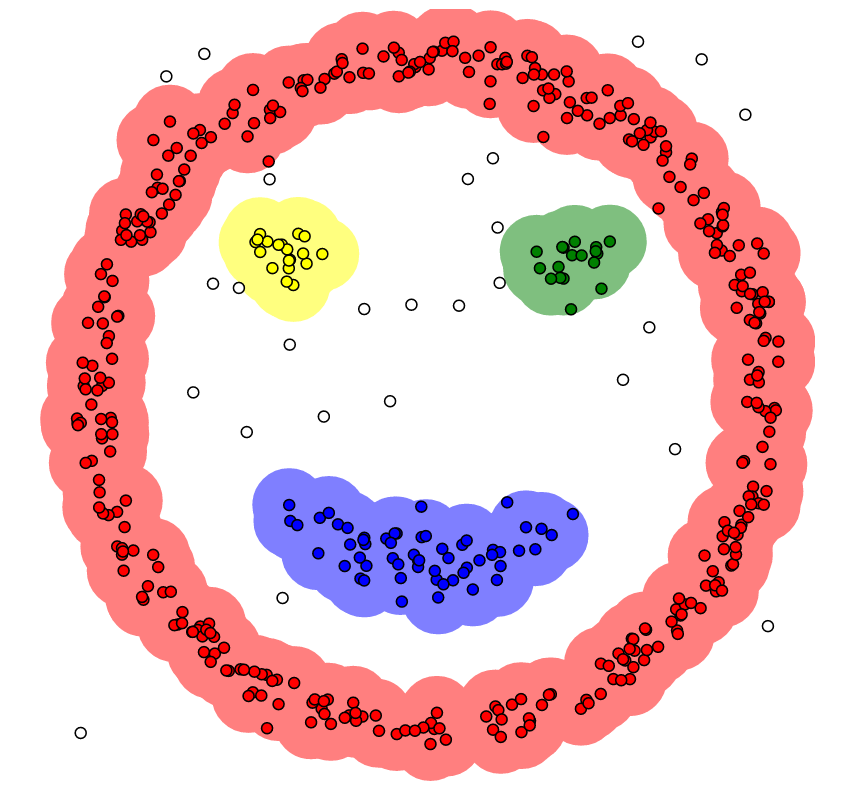
\includegraphics[width=0.6\linewidth]{Rysunki/Rozdzial2/dbscan.png}
    \caption{Przynależność punktów do klastrów w algorytmie DBSCAN}
    \label{fig:dbscan}
    \end{figure}
    
    
\section{Weryfikacja danych}
    \subsection{Histogram} \label{sec:histogram}
    Histogram jest jednym ze sposobów przedstawienia rozkładu empirycznego. Posiada on oś $x$, na której są położone słupki pewnych grup lub cech z danego zbioru danych. Oś $y$ reprezentuje ilość wystąpień danej grupy lub cechy. Histogram można wykorzystać na przykład do prezentacji ilości wystąpień słów we wszystkich dokumentach tekstowych z jednej grupy. Dzięki takiemu przedstawieniu można łatwo określić jaka grupa tych dokumentów posiada jaką tematykę. W niniejszej pracy histogram jest wykorzystywany, aby określić ilość wystąpień klas zwróconych przez algorytm klasteryzacji, względem klas rzeczywistych tych samych dokumentów tekstowych.
    \begin{figure}[h!]
        \centering
    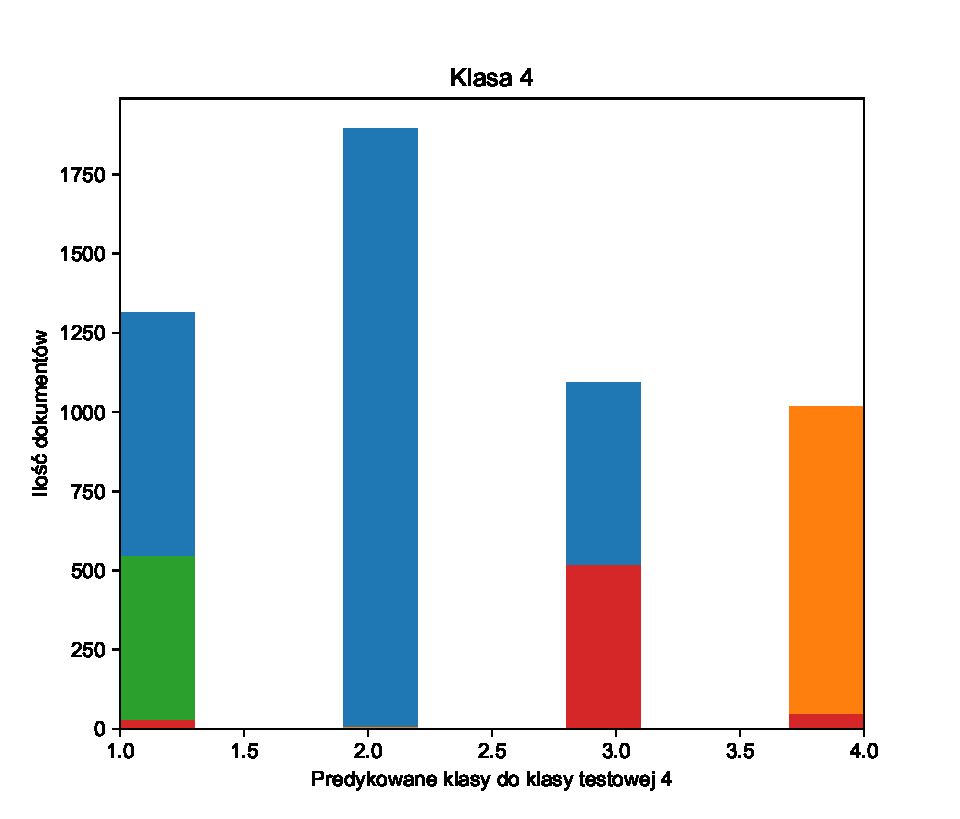
\includegraphics[width=0.7\linewidth]{Rysunki/Rozdzial2/Figure_2.pdf}
    \caption{Przykładowy histogram}
    \label{fig:histogram}
    \end{figure}
    
    \newpage
    
    \subsection{Macierz pomyłek} \label{sec:confusion}
    Macierz pomyłek jest narzędziem stosowanym do oceny jakości wyników z algorytmu klasteryzacji. Na osi $x$ znajdują się etykiety klas, które wyznaczane są przez algorytm klasteryzacji, a na osi $y$ rzeczywiste etykiety klas. 
    \begin{figure}[h!]
        \centering
    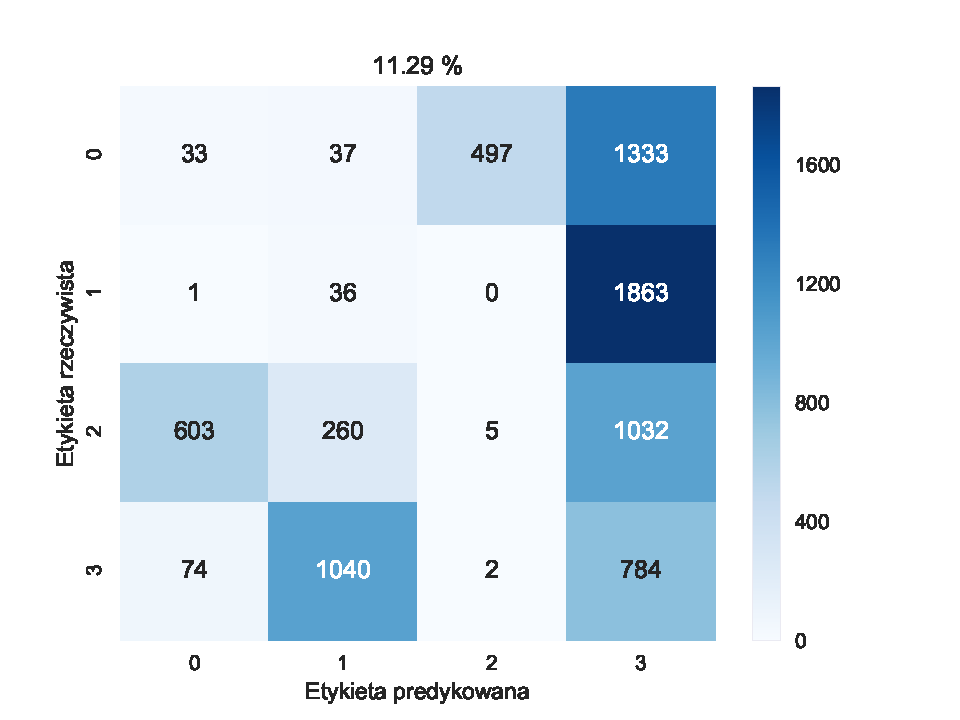
\includegraphics[width=0.7\linewidth]{Rysunki/Rozdzial2/confusion.pdf}
    \caption{Przykładowa macierz pomyłek}
    \label{fig:confugsion}
    \end{figure}
    
    Odczytanie danych z macierzy pomyłek z \ref{fig:confugsion} następuje w taki sposób, że każdy wiersz to klasa rzeczywista analizowanych dokumentów tekstowych. Kolumny oznaczają klasy, które wyznaczył algorytm klasteryzacji. 
    Z macierzy przedstawionej na rysunku \ref{fig:confugsion} możemy odczytać, że dla 33 dokumentów tekstowych mających przypisaną etykietę rzeczywistą "0", algorytm również znalazł oraz przypisał taką samą etykietę.
    
    \newpage
    \subsection{Kombinacje klas predykowanych we wszystkich możliwościach} \label{sec:zamianaKlas}
    Wygenerowanie wszystkich kombinacji przypisań klas predykowanych, pozwoli na znalezienie najlepszego mapowania do klas rzeczywistych. Algorytmy klasteryzacji należą do technik uczenia nienadzorowanego. Z tego względu podczas wielokrotnego uruchamiania algorytmu, pogrupowane dokumenty tekstowe mogą raz znaleźć się w klastrze o etykiecie "1", a innym razem w klastrze "4". By zweryfikować dokładność klasteryzacji potrzebne jest dopasowanie etykiet przypisanych przez algorytm do etykiet rzeczywistych. 
    
    W tym celu stosuje się zamiany klas wygenerowanych przez algorytm w różnych kombinacjach. Schemat działania zamiany klas wygląda w taki sposób, że należy wziąć wyjściową listę etykiet z algorytmu (na \ref{tab:kombinacje} jest to 1 kombinacja), utworzyć macierz pomyłek oraz policzyć trafność przypisania klas (ang. accuracy). Następnie przesunąć każdą predykowaną klasę o jedną klasę w przód, aż do momentu uzyskania początkowych wyników. Dla każdego przypadku liczymy trafność przypisania klas. Wybieramy takie przypisanie, w którym trafność w skali procentowej jest największa.
    \begin{table}[h!]
    \centering
    \caption{Przykładowe kombinacje dla etykiet predykowanych}
    \label{tab:kombinacje}
    \begin{tabular}{|l|l|l|l|}
    \hline
    1 kombinacja & 2 kombinacja & 3 kombinacja & 4 kombinacja \\ \hline
    4           & 1            & 2            & 3            \\ \hline
    4           & 1            & 2            & 3            \\ \hline
    2           & 3            & 4            & 1            \\ \hline
    4           & 1            & 2            & 3            \\ \hline
    1           & 2            & 3            & 4            \\ \hline
    3           & 4            & 1            & 2            \\ \hline
    3           & 4            & 1            & 2            \\ \hline
    2           & 3            & 4            & 1            \\ \hline
    3           & 4            & 1            & 2            \\ \hline
    4           & 1            & 2            & 3            \\ \hline
    \end{tabular}
    \end{table}
\chapter{Opis i wyniki przeprowadzonych testów}

\section{Przebieg procesu testowania}
Część praktyczna pracy polegała na implementacji programu do klasteryzacji dokumentów tekstowych oraz przeprowadzeniu testów weryfikujących skuteczność opracowanego rozwiązania. Opracowany system na wejściu otrzymuje listę dokumentów tekstowych w postaci pliku ".csv", a w rezultacie tworzy nowy plik ".csv" z listą dokumentów tekstowych oraz przypisanymi do nich etykietami klastrów. Przygotowanie takiego projektu składało się z kilku etapów:
\begin{itemize}
    \item znalezienie dużego zbioru dokumentów tekstowych potrzebnego do przeprowadzenia testów weryfikujących skuteczność systemu,
    \item przetworzenie dokumentów tekstowych na format akceptowalny przez procedury wykorzystane do implementacji klasteryzacji,
    \item implementacja systemu do wstępnego przetwarzania i klasteryzacji dokumentów tekstowych,
    \item przeprowadzenie testów weryfikujących skuteczność wybranej metody klasteryzacji.
\end{itemize}
\newpage

Celem eksperymentu jest znalezienie jak najbardziej podobnych do siebie dokumentów, korzystając tylko z metod przetwarzania dokumentów tekstowych oraz klasteryzacji. W pracy zostały wykorzystane takie metody jak, "stemming", "tf-idf".

Problem polega na tym, że klasteryzacja, inaczej zwana klasyfikacją nienadzorowaną, zwraca podzielone dokumenty na grupy w różny sposób. Interpretacja wygenerowanych klastrów wymaga zastosowania kilku metod w celu weryfikacji czy dany wynik jest poprawny bądź nie. Dokumenty tekstowe znajdujące się w zbiorze testowym posiadają etykiety opisujące ich przynależność do predefiniowanych klas. Zatem weryfikacja skuteczności klasteryzacji będzie polegała na porównaniu dla każdego dokumentu jego klasy referencyjnej z klasą przypisaną mu przez algorytm klasteryzacji.

\section{Wykorzystane dane do przeprowadzenia eksperymentów}
Do przeprowadzenia eksperymentów został wykorzystany zbiór danych znalezionych na jednej ze stron internetowych \cite{datasetclass} o nazwie roboczej \texttt{"ag\_news\_csv"}. Dokumenty tekstowe zawarte w tym zbiorze są podzielone na 4 grupy.

\begin{table}[h!]
    \centering
    \caption{Klasy z danego zbioru danych}
    \label{datasetclasses}
    \begin{tabular}{|l|l|l|l|l|}
    \hline
    Numer klasy & 1     & 2      & 3        & 4        \\ \hline
    Nazwa klasy & World & Sports & Business & Sci/Tech \\ \hline
    \end{tabular}
\end{table}

Zbiór danych zawiera w sobie dwa pliki \texttt{"test.csv"} oraz \texttt{"train.csv"}. Ilość dokumentów dla obu plików jest różna i prezentuje się w taki sposób:

\begin{table}[h!]
    \centering
    \caption{Ilość dokumentów tekstowych w poszczególnych klasach i zbiorach danych}
    \label{quantityOfDocs}
    \begin{tabular}{|l|l|l|}
    \hline
    Numer klasy & test.csv & train.csv \\ \hline
    1           & 1900     & 30000     \\ \hline
    2           & 1900     & 30000     \\ \hline
    3           & 1900     & 30000     \\ \hline
    4           & 1900     & 30000     \\ \hline
    \end{tabular}
\end{table}
Struktura w pliku z danymi źródłowymi jest taka, że każda nowa linia to osobny dokument tekstowy. Informacje rozdzielone są separatorem przecinka. W pliku są trzy informacje, takie jak numer klasy oryginalnej, nazwa artykułu oraz treść artykułu. 

Powodem dla którego został wybrany ten zbiór danych, jest fakt, że zbiór ten nie posiada dużo klas, dzięki czemu stopień trudności klasteryzacji jest mniejszy. Wydobycie cech z dokumentów tekstowych w podanym zbiorze, możliwe jest dzięki odpowiedniej długości słów w nich zawartych.

W wypadku, gdy dokument tekstowy będzie zbyt krótki, po całym procesie przetwarzania może nie mieć ani jednej cechy opisującej ten dokument. Cechami w tym przypadku są częstości występowania słów kluczowych, których lista ustalana jest w wyniku przetwarzania wstępnego wszystkich tekstów.


Podczas analizowania treści tych dokumentów, napotkałem na wiele różnych elementów, które nie wnoszą nic do ich istotności. Są to m.in. adresy URL, akronimy, czy elementy znaczników HTML, ponieważ dokumenty tekstowe w podanym zbiorze pochodzą ze stron internetowych, dlatego w kilku przypadkach parsowanie i kasowanie HTML nie zadziałało poprawnie. Takie elementy mogą zakłócić działanie algorytmu. Bardzo ważny jest moment przetwarzania dokumentów tekstowych, tak by zostały w nim tylko istotne słowa.
\newpage

\section{Cele szczegółowe}
    \subsection{Parsowanie HTML}
    Niektóre dokumenty z podanego zbioru posiadają w sobie różnego rodzaju znaczniki HTML czy nawet adresy URL, które są zbędnymi słowami jeśli chodzi o klasteryzację. W tym celu została napisana metoda, która przyjmuje treść dokumentu tekstowego jako parametr i zwraca ten sam dokument bez znaczników i znaków specjalnych takich jak "\&lt;". Metody te korzystają z bibliotek "html" oraz "re" dostarczonych przez język Python.
    
    \lstinputlisting[label={lst:3.4},caption={Metody do kasowania znaczników HTML oraz adresów URL}, language=python, showstringspaces=false, breaklines=true]{Algorytmy/Rozdzial3/parsehtml.py}   
    
    Obie metody można wykorzystać w funkcji "PrepareDocument", która została zaprezentowana w rozdziale \ref{lst:3.2}.
    
    Metoda "RemoveHTMLTags" przyjmuje jako parametr dokument tekstowy. W pierwszej kolejności korzysta z metody "html.unescape", która zamienia wszystkie znaki specjalne (np. \&gt;, \&\#62;), na ich odpowiedniki w formacie Unicode.  Następnie poprzez użycie wyrażeń regularnych usuwa znaczniki HTML, bez kasowania ich zawartości. Metoda "RemoveUrl" również przyjmuje dokument tekstowy jako parametr. Korzystając z wyrażenia regularnego na danym tekście, wszystkie znalezione wzorce są zamieniane na pusty tekst.
    
    
    \subsection{Schemat działania algorytmu} \label{sec:alg}
    \begin{figure}[h!]
        \centering
        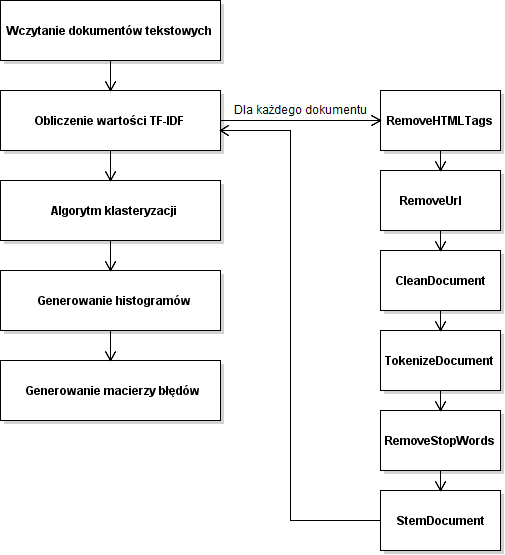
\includegraphics[scale=0.6]{Rysunki/Rozdzial3/diagram.png}
        \caption{Diagram przedstawiający etapy działania programu do klasteryzacji dokumentów tekstowych}
        \label{fig:diagram}
    \end{figure}
    Na samym początku należy skonfigurować algorytm, tak by działał z odpowiednimi danymi. W przypadku algorytmu k-means należy określić, na ile klas chcemy podzielić dane. Należy również określić ścieżkę dostępu do pliku \texttt{".csv"} ze zbiorem danych, oraz nazwami klas. Kolejnym etapem jest pobranie wszystkich dokumentów tekstowych do listy.
    \newpage
    \lstinputlisting[label={lst:3.1},caption={Pobieranie dokumentów tekstowych z pliku .csv}, language=python, showstringspaces=false, breaklines=true]{Algorytmy/Rozdzial3/getFile.py}
    
    Dalej, wszystkie dokumenty są przygotowywane zgodnie z wymaganiami. Przygotowanie dokumentu tekstowego dzieli się na 4 etapy:
    \begin{enumerate}
        \item czyszczenie (patrz \ref{sec:czyszczenie}),
        \item tokenizacja (patrz \ref{sec:tokenizacja}),
        \item usuwanie słów zawartych w stop liście ,
        \item normalizacja, czyli stemming (patrz \ref{sec:normalizacja}).
    \end{enumerate}
    
    \lstinputlisting[label={lst:3.2},caption={Implementacja metod odpowiedzialnych za przygotowanie dokumentów tekstowych}, language=python, showstringspaces=false, breaklines=true]{Algorytmy/Rozdzial3/prepareDoc.py}
    
    Parametr "tokenizer" wymusza wykorzystanie naszej metody do celów tokenizacji, który dodatkowo ma zaimplementowane inne elementy przygotowania dokumentu tekstowego. Na samym końcu uruchomiamy algorytm klasteryzacji.
    \lstinputlisting[label={lst:3.3},caption={Uruchomienie algorytmu k-Means}, language=python, showstringspaces=false, breaklines=true]{Algorytmy/Rozdzial3/kmeans.py}
    
    Algorytm k-means \ref{sec:kmeans} w bibliotece Scikit-learn zwraca listę przypisanych klas do dokumentów tekstowych w takiej samej kolejności, w jakiej otrzymał je na wejściu.
    
    \subsection{Weryfikacja poprawności rezultatów}
    Algorytm klasteryzacji ma jedną istotną wadę: numery klastrów, które zostały zwrócone, nie muszą odzwierciedlać faktycznych klas dokumentów tekstowych. Dlatego też ważnym elementem jest poprawna weryfikacja jakości wyników. W pracy opisane zostaną dwie metody weryfikacji zwróconych klas. 
    
    Dokumenty tekstowe ze zbioru danych posiadają już przypisaną klasę do każdego dokumentu. Ta wiedza jest istotna podczas generowania macierzy pomyłek \ref{sec:confusion}. Weryfikacja dokładności klasyfikacji dokumentów za pomocą klasteryzacji odbywa się kilkuetapowo:
    
    \begin{itemize}
        \item wygenerowanie macierzy pomyłek, dla predykowanych klas wygenerowanych za pomocą algorytmu klasteryzacji,
        \item wygenerowanie histogramu z rozkładem klas w poszczególnych klastrach,
        \item zmapowanie na nowo predykowanych klas, korzystając z informacji z histogramu, oraz wygenerowanie macierzy pomyłek,
        \item zmapowanie predykowanych klas na wszystkie sposoby prezentacji, wygenerowanie dla każdej kombinacji macierzy pomyłek, oraz policzenie trafności przypisanych klas.
    \end{itemize}
\newpage
\section{Wyniki testów}
    Wykorzystując przedstawione w poprzednim punkcie kroki, istnieje możliwość zbadania wyników klasteryzacji na danym zbiorze danych \texttt{"ag\_news\_csv"}. 
    
    Na początku zostały przedstawione wyniki z pierwszego uruchomienia algorytmu na pliku "test.csv", który zawiera po 1900 dokumentów tekstowych z każdego klastra.
    
    Uruchomienie programu na zbiorze testowym, wyświetli 4 wykresy w osobnych oknach. Wykresy zostały przedstawione oraz omówione na rysunkach \ref{fig:r11}, \ref{fig:r12}, \ref{fig:r13} i \ref{fig:r15}.
    
    \begin{figure}[h!]
        \centering
        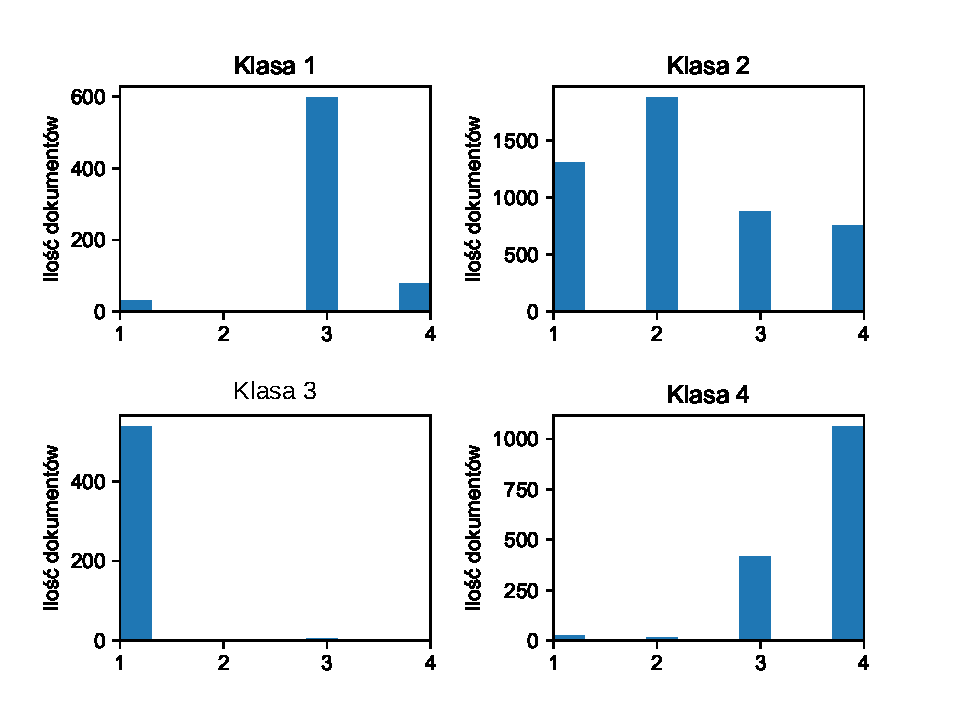
\includegraphics[scale=0.8]{Rysunki/Rozdzial3/edited_run11.pdf}
        \caption{Uruchomienie 1: Histogram}
        \label{fig:r11}
    \end{figure}
    
    Wygenerowane na powyższym rysunku \ref{fig:r11} histogramy, odzwierciedlają ilość przypisanych klas przez algorytm klasteryzacji do dokumentów tekstowych należących do predefiniowanej klasy.
    
    Poniższy rysunek \ref{fig:r12} przedstawia macierz błędu. Został on wygenerowany na podstawie etykiet rzeczywistych oraz predykowanych zwróconych przez algorytm klasteryzacji.
    
    \begin{figure}[h!]
        \centering
        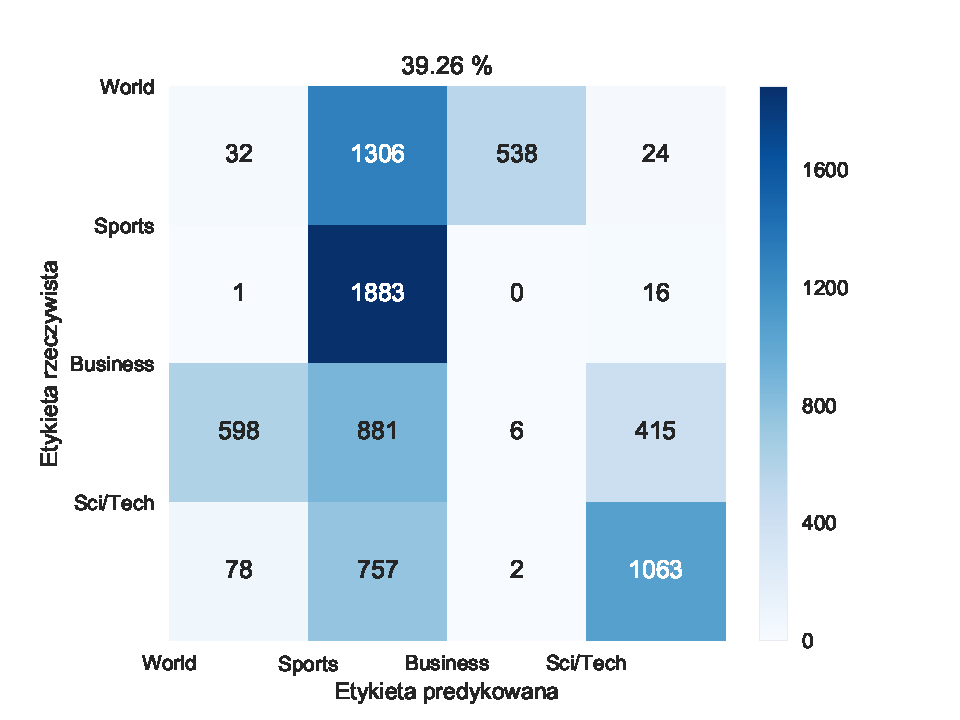
\includegraphics[scale=0.6]{Rysunki/Rozdzial3/run12.pdf}
        \caption{Uruchomienie 1: Macierz błędu dla danych zwróconych z algorytmu}
        \label{fig:r12}
    \end{figure}
    
    \newpage
    Nazwą macierzy jest policzona metryka trafności (ang. accuracy) wyników. Idealne uruchomienie posiadałoby trafność na poziomie 100 \%, a macierz miałaby wszystkie dokumenty tekstowe znalezione po przekątnej. Na tym etapie wynik poprawności algorytmu klasteryzacji dla tego zbioru danych to 39.26 \%. 
    
    Można jednak spróbować zrobić nowe mapowanie klas odkrytych przez algorytm, dzięki wcześniej wygenerowanemu histogramowi \ref{fig:r11}. Zakładając, że dla dokumentów z klasy "1" algorytm przypisał nowe etykiety, to uznać można, że klasa predykowana "3" jest naszą oryginalną "1". Tak samo postępujemy z kolejnymi histogramami. Dzięki temu można przyjąć nowe mapowanie klas. 
    
    \begin{table}[h!]
        \centering
        \caption{Uruchomienie 1: Nowe mapowanie klas predykowanych}
        \label{newMapPred}
        \begin{tabular}{|l|l|}
        \hline
        Jaka klasa & Predykowana klasa \\ \hline
        1          & 3                 \\ \hline
        2          & 2                 \\ \hline
        3          & 1                 \\ \hline
        4          & 4                 \\ \hline
        \end{tabular}
    \end{table}
    
    W przedstawionym przypadku należy zamienić wszystkie "3" na "1" oraz "1" na "3". Takie mapowanie utworzy nową listę etykiet, a macierz błędu wyglądać będzie następująco:
    \newpage
    \begin{figure}[h!]
        \centering
        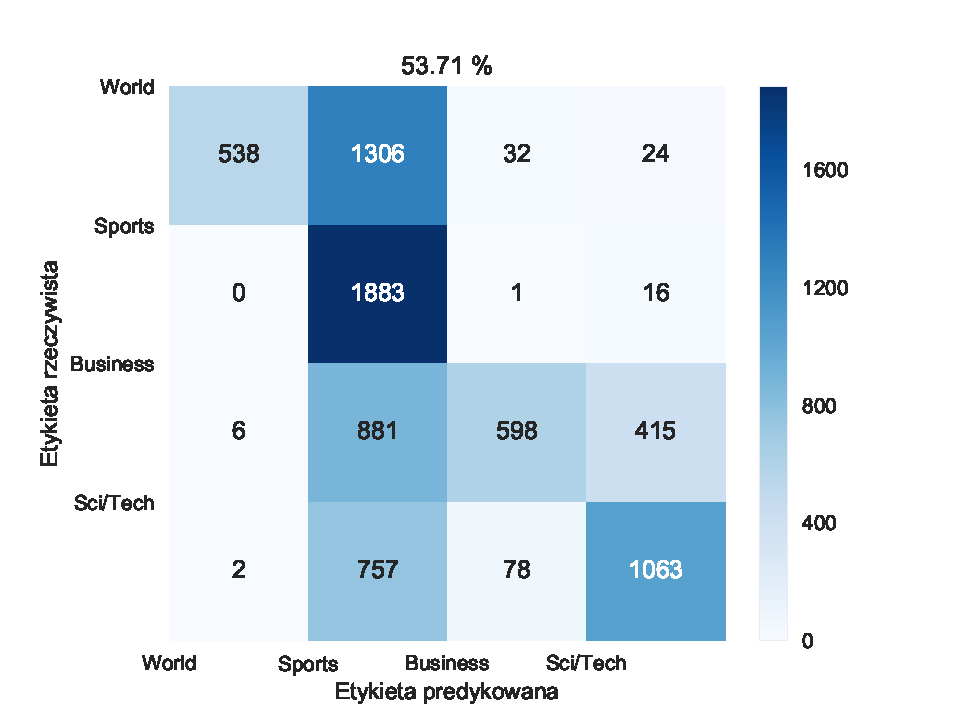
\includegraphics[scale=0.57]{Rysunki/Rozdzial3/run13.pdf}
        \caption{Uruchomienie 1: Macierz błędu dla danych po zmapowaniu etykiet z histogramów}
        \label{fig:r13}
    \end{figure}    
    
    Takie mapowanie klas, zwiększyło trafność, aż do 53.71 \%. 
    
    Na koniec należy skorzystać jeszcze z jednej opcji weryfikacji poprawności danych. Zamiana predykowanych klas w różnych kombinacjach przedstawiona została w \ref{sec:zamianaKlas}. Mapowanie w ten sposób klas pokazało, że takie kombinacje nie są na tyle dobre, aby uznać je za poprawne. Dzieje się tak chociażby ze względu na to, że mapowanie z histogramu dało lepszy rezultat.
    
    \begin{figure}[h!]
        \centering
        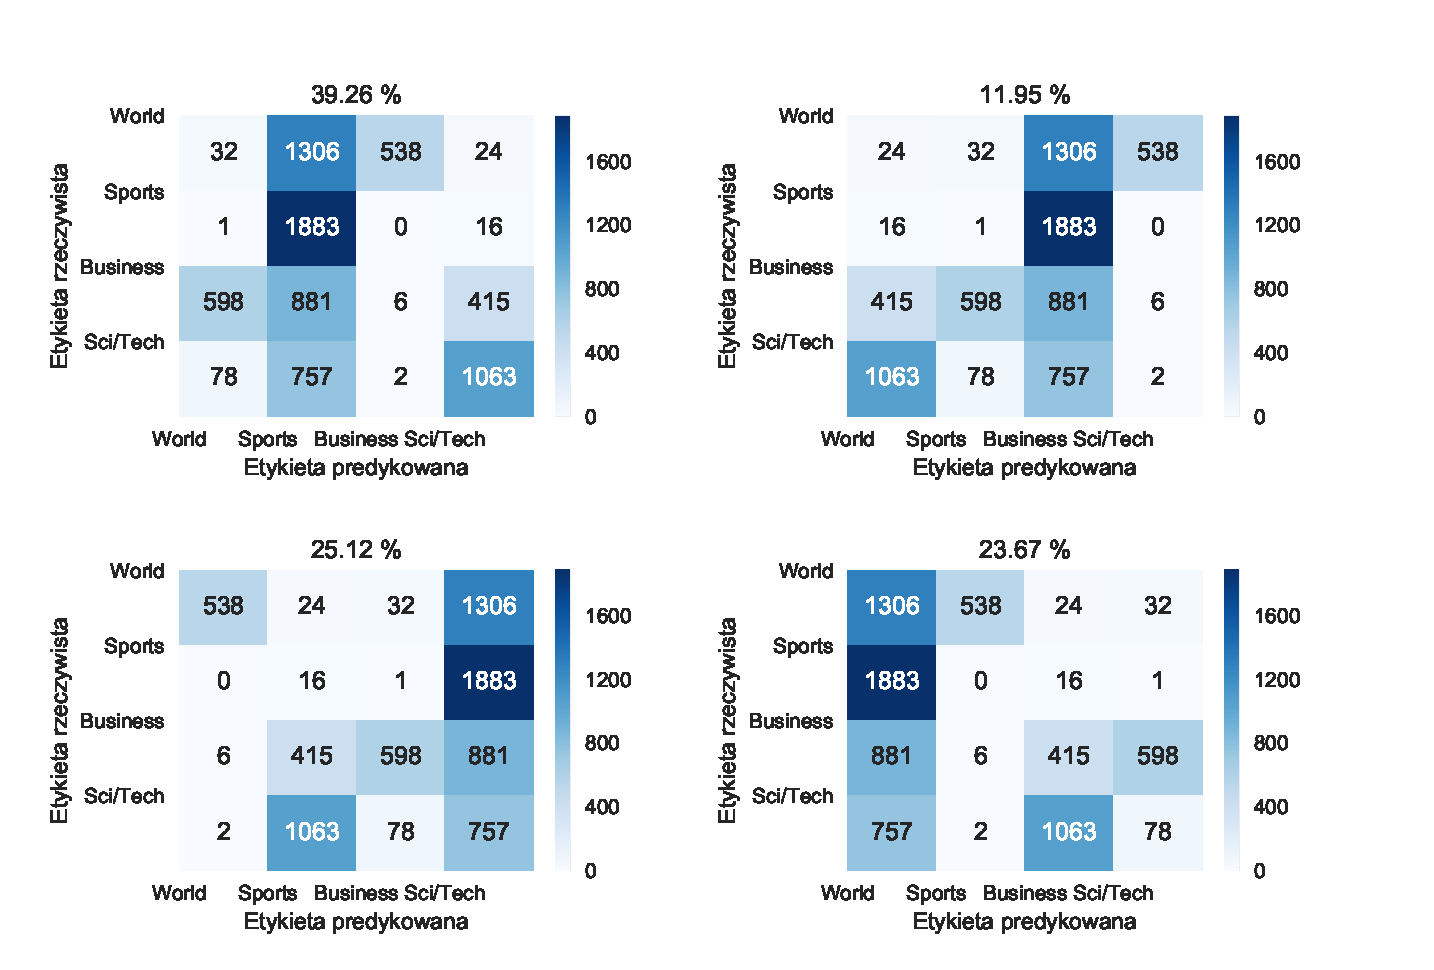
\includegraphics[scale=0.57]{Rysunki/Rozdzial3/run15.pdf}
        \caption{Uruchomienie 1: Macierze błędów po dokonaniu zamiany klas}
        \label{fig:r15}
    \end{figure}
    Dla pierwszego uruchomienia, przypisanie klas z \ref{newMapPred} jest najlepszym mapowaniem.
    Na tych danych algorytm klasteryzacji został uruchomiony 5 razy, na trzech różnych progach ilości przeprowadzonych iteracji: 10, 100 i 400. Tak prezentują się wyniki poszczególnych uruchomień.
    \begin{table}[h!]
        \centering
        \caption{Najlepsze wyniki dla 5 uruchomień na zbiorze danych "test"}
        \label{bestAccTest}
        \begin{tabular}{|c|c|c|c|}
        \hline
        Lp. & \begin{tabular}[c]{@{}c@{}}Najlepsza trafność \\ dla 10 iteracji\end{tabular} & \begin{tabular}[c]{@{}c@{}}Najlepsza trafność \\ dla 100 iteracji\end{tabular} & \begin{tabular}[c]{@{}c@{}}Najlepsza trafność \\ dla 400 iteracji\end{tabular} \\ \hline
    1 & 53.38 \% - Zamiana klas & 50.63 \% - Histogram & 53.71 \% - Histogram \\ \hline
    2 & 62.38 \% - Zamiana klas & 58.92 \% - Histogram & 53.62 \% - Histogram \\ \hline
    3 & 33.33 \% - Zamiana klas & 52.86 \% - Histogram & 53.34 \% - Zamiana klas \\ \hline
    4 & 64.07 \% - Zamiana klas & 52.76 \% - Zamiana klas & 53.33 \% - Histogram \\ \hline
    5 & 37.75 \% - Zamiana klas & 59.68 \% - Histogram & 59.95 \% - Histogram \\ \hline
        \end{tabular}
    \end{table}
    
    Średnie procentowe wyniki trafności na wyznaczonych progach są do siebie dość podobne. Dla 10 iteracji średnia trafności jest mniejsza o 4 punkty procentowe. Można również zauważyć pewną zależność: czym mniej iteracji tym lepsza trafność prezentowana była w sposobie weryfikacji zamiany klas. Natomiast w liczbie iteracji od 100 do 400, sposób mapowania zwykle opierał się na bazie histogramu.
    
    Zastosowanie sposobów weryfikacji na zbiorze danych zawierających 30000 dokumentów tekstowych dało gorsze wyniki przy uruchomieniu na 10 iteracjach.
    \begin{table}[h!]
        \centering
        \caption{Najlepsze wyniki dla 3 uruchomień na zbiorze danych "train"}
        \label{bestAccTrain}
        \begin{tabular}{|c|c|c|c|}
        \hline
        Lp. & \begin{tabular}[c]{@{}c@{}}Najlepsza trafność \\ dla 10 iteracji\end{tabular} & \begin{tabular}[c]{@{}c@{}}Najlepsza trafność \\ dla 100 iteracji\end{tabular} & \begin{tabular}[c]{@{}c@{}}Najlepsza trafność \\ dla 400 iteracji\end{tabular} \\ \hline
        1 & 38.66 \% - Zamiana klas & 51.7 \% - Histogram & 34.53 \% - Zamiana klas \\ \hline
        2 & 33.45 \% - Zamiana klas & 34.54 \% - Zamiana klas & 51.77 \% - Zamiana klas \\ \hline
        3 & 43.72 \% - Zamiana klas & 51.8 \% - Zamiana klas & 51.66 \% - Zamiana klas \\ \hline
        \end{tabular}
    \end{table}
\chapter{Podsumowanie}

W pracy zostały poruszone tematy związane z analizą tekstu oraz grupowaniem dokumentów tekstowych, wykorzystując w tym celu metody czyszczenia, normalizacji oraz reprezentacji tekstu za pomocą miary $TF-IDF$. Na dzień dzisiejszy, analizowanie dokumentów tekstowych jest dość trudnym zagadnieniem.  Oprócz samej budowy zdań w tekście, należy również rozumieć sens słów, ponieważ w niektórych sytuacjach to właśnie sens słowa jest istotniejszym elementem, decydującym o przynależności dokumentu do konkretnej grupy tekstów. 

Praca ta prezentuje poszczególne kroki podjęte dla osiągnięcia celu. Omówione zostały pojęcia teoretyczne konkretnych technologii, instalacja oraz konfiguracja środowiska pracy Visual Studio Code oraz języka programowania Python. Opisane zostały możliwości wykorzystywanych bibliotek do wstępnego przetwarzania tekstu.

W kolejnych częściach pracy przedstawione zostały etapy przygotowań dokumentów tekstowych do wykorzystania podczas grupowania tekstu, oraz algorytm, który został wykorzystany do osiągnięcia zamierzonego celu.

Aby dokonać weryfikacji dokładności klasteryzacji dokumentów tekstowych opracowano metodę dopasowywania klastrów wygenerowanych przez algorytm k-means do etykiet referencyjnych. Do tego celu wykorzystane zostało przedstawienie danych na histogramach, oraz zamiana klas wyjściowych z wykorzystaniem różnych mapowań.

Przedstawiony w niniejszej pracy system jest możliwy do uruchomienia na innych zbiorach dokumentów tekstowych. Przykładowe zbiory takich dokumentów dostępne są w załączniku na płycie CD dołączonej do pracy.


%\begin{appendix}
%	\appendix
%	\chapter{Cel dodatków w pracy}
%=================================================================================================
Do materiałów, które mogą uzupełnić pracę, oprócz rysunków, tablic, ilustracji
itp. należą także dodatki, nazwane również aneksami. Dają one możliwość albo
dołączenia do tekstu głównego różnorodnego rodzaju informacji dodatkowych, albo
wyłączenia z tekstu głównego tych wiadomości, które nie są w nim konieczne. Niekiedy
pewne wiadomości wplecione w tekst niepotrzebnie go obciążają, przerywają
zasadniczy wątek lub są nadmiernie szczegółowe. Jeśli mimo to wiadomości te są
użyteczne i mogą być przydatne, warto oczyścić z nich tekst główny i zgrupować je
na końcu pracy w postaci dodatków.

Przykładem użycia dodatków może być opis zawartości płyty CD lub DVD dołą-
czonej do pracy lub instrukcje laboratoryjne stworzone w oparciu o napisaną pracę.

%=================================================================================================

%	\chapter{Składanie wzorów}
W tej części nie opisywano już samych zasad tworzenia dokumentu, a zamiast
tego skupiono się na przedstawieniu kilku przykładowo złożonych wzorów. W źró-
dłach szablonu możliwe jest sprawdzenie jak wzór był pisany z wykorzystaniem notacji
\LaTeX oraz pakietu \AmS. Więcej szczegółów zawiera rozdział ósmy świetnego
opracowania e{companion:04} oraz dokumentacja pakietu

\begin{itemize}
\item Wzór dzielony i wyrównywany do znaku
\begin{equation}
	\begin{split}
		(a+b)^4  &= (a+b)^2 (a+b)^2 \\
					&= (a^2+2ab+b^2)(a^2+2ab+b^2) \\
					&= a^4+4a^3b+6a^2b^2+4ab^3+b^4. \\
	\end{split}
\end{equation}

\item Wzór w kilku liniach
\begin{multline}
	a+b+c+d+e+f+g+h+i+j+k+l+m+n\\
							o-p-r-s-t-u-w-x-y-z.
\end{multline}

\item Grupa wzorów
\begin{gather}
	a_1=b_1+c_1,\\
	a_2=b_2+c_2-d_2+e_2.
\end{gather}
\item Wzory z wyrównywaniem do znaku i osobną numeracją
\begin{align}
	x^2+y^2	&= 1, 					& x^3+y^3	&=1, \\
				x&=\sqrt{1-y^2},	& x 			&= \sqrt[3]{1-y^3}.
\end{align}

\begin{align}
	a_{11}& =b_{11},&
	a_{12}& =b_{12},\\
	a_{21}& =b_{21},&
	a_{22}& =b_{22}+c_{22}.
\end{align}
\item Wzory z wyrównywaniem do znaku oraz zewnętrznych marginesów i osobną numeracją 
\begin{flalign}
	a_{11}&	=b_{11},&
	a_{12}&	=b_{12},\\
	a_{21}&	=b_{21},&
	a_{22}&	=b_{22}+c_{22}.
\end{flalign}

\item Klamra
\begin{equation}
P_{r-j}=\begin{cases}
	0							& \text{jeśli $r-j$ jest nieparzyste},\\
	r!\,(-1)^{(r-j)/2}	& \text{w przeciwnym razie}.
\end{cases}
\end{equation}

\item Macierze
\begin{equation}
A=
	\begin{bmatrix}
		a	&	b	&	c		&	d	\\
		b	&	a	&	c+d	&	c-d	\\
		0	&	0	&	a+b	&	a-b	\\
		0	&	0	&	ab		&	cd	\\
	\end{bmatrix},
\end{equation}

\begin{equation}I_4=
	\begin{pmatrix}
			1 & 0 & 0 & 0 \\
		 	0 & 1 & 0 & 0 \\
			0 & 0 & 1 & 0 \\
			0 & 0 & 0 & 1 \\ 
	\end{pmatrix}
,\quad
\det{I_4}=
	\begin{vmatrix}
			1 & 0 & 0 & 0 \\
		 	0 & 1 & 0 & 0 \\
			0 & 0 & 1 & 0 \\
			0 & 0 & 0 & 1 \\ 
	\end{vmatrix}.
\end{equation}

\item Granica
\begin{equation}
\lim_{x\to 0}(1+x)^{\frac{1}{x}}=\mathrm{e}.
\end{equation}
\item Całka
\begin{equation}
\int_{0}^{1}3x^2\,\mathrm{d}x.
\end{equation}
\item Wzór z funkcjami trygonometrycznymi
\begin{equation}
\sin (\alpha \pm \beta) = \sin (\alpha) \cdot \cos (\beta) \pm \cos (\alpha) \cdot \sin (\beta).
\end{equation} 

\item Wzór Taylora
\begin{equation}
	\begin{split}f(x) &= f(a) + \frac{x-a}{1!} f^{(1)}(a) + \frac{(x-a)^2}{2!} f^{(2)}(a) + \ldots \\
							&+ \frac{(x-a)^n}{n!} f^{(n)}(a) + R_n(x,a)\\
							&= \sum\limits_{k=0}^n \left( \frac{(x-a)^k}{k!} f^{(k)}(a) \right) + R_n(x,a).
	\end{split}
\end{equation}
\end{itemize}

%\end{appendix}

\begin{flushleft}
	\bibliography{Bibliografia/bibliografia}
\end{flushleft}

\end{document}